\section{Einleitung} \label{zeta:section:einleitung}
\kopfrechts{Einleitung}

Die Riemannsche Zeta-Funktion $\zeta(s)$ ist für alle komplexe $s$ mit $\Re(s) > 1$ definiert als
\index{Zeta-Funktion, Riemannsche}%
\begin{equation}\label{zeta:equation1}
    \zeta(s)
    =
    \sum_{n=1}^{\infty}
    \frac{1}{n^s}.
\end{equation}
Die Zeta-Funktion ist bekannt als Bestandteil der Riemannschen Vermutung, welche besagt das alle nichttrivialen Nullstellen der Zeta-Funktion einen Realteil von $\frac{1}{2}$ haben.
\index{Riemannsche Vermutung}%
Mithilfe dieser Vermutung kann eine gute Annäherung an die Primzahlfunktion gefunden werden.
\index{Primzahlfunktion}%
Die Primzahlfunktion steigt immer an, sobald eine Primzahl vorkommt.
Eine Darstellung davon ist in Abbildung \ref{fig:zeta:primzahlfunktion} zu finden.
Die Riemannsche Vermutung ist eines der ungelösten Millennium-Probleme der Mathematik, auf deren Lösung eine Belohnung von einer Million Dollar ausgesetzt ist \cite{zeta:online:millennium}.
\index{Millennium-Problem}%
Auf eine genauere Beschreibung der Riemannschen Vermutung wird im Rahmen dieses Papers nicht eingegangen.
\begin{figure}
    \centering
%    %
% primzahlfunktion2.tex -- Primzahlfunktion, alternativer Vorschlag
%
% (c) 2021 Prof Dr Andreas Müller, OST Ostschweizer Fachhochschule
%
\documentclass[tikz]{standalone}
\usepackage{amsmath}
\usepackage{times}
\usepackage{txfonts}
\usepackage{pgfplots}
\usepackage{csvsimple}
\usetikzlibrary{arrows,intersections,math}
\begin{document}
\def\skala{1}
\begin{tikzpicture}[>=latex,thick,scale=\skala]

\def\dx{0.38}
\def\dy{0.5}

\foreach \x in {1,...,30}{
	\draw[color=gray!20] ({\x*\dx},0) -- ({\x*\dx},{10.5*\dy});
}
\foreach \y in {1,...,10}{
	\draw[color=gray!20] (0,{\y*\dy}) -- ({30.5*\dx},{\y*\dy});
}

\draw[->] (-0.1,0) -- ({30.8*\dx},0) coordinate[label={$x$}];
\draw[->] (0,-0.1) -- (0,{10.9*\dy}) coordinate[label={right:$\pi(x)$}];

\def\segment#1#2#3{
	%\draw[line width=0.1pt] ({#3*\dx},0) -- ({#3*\dx},{#2*\dy});
	\draw[color=blue,line width=1.4pt]
		({#1*\dx},{#2*\dy}) -- ({#3*\dx},{#2*\dy});
	\draw[color=blue,line width=0.3pt]
		({#3*\dx},{#2*\dy}) -- ({#3*\dx},{(#2+1)*\dy});
	\draw ({#3*\dx},-0.1) -- ({#3*\dx},0.1);
	\node at ({(#3)*\dx},-0.1) [below] {$#3\mathstrut$};
}

\foreach \y in {2,4,...,10}{
	\draw (-0.1,{\y*\dy}) -- (0.1,{\y*\dy});
	\node at (-0.1,{\y*\dy}) [left] {$\y\mathstrut$};
}

\begin{scope}
\clip (0,-0.5) rectangle ({30*\dx},{10.1*\dy});

\segment{0}{0}{2}
\segment{2}{1}{3}
\segment{3}{2}{5}
\segment{5}{3}{7}
\segment{7}{4}{11}
\segment{11}{5}{13}
\segment{13}{6}{17}
\segment{17}{7}{19}
\segment{19}{8}{23}
\segment{23}{9}{29}
\segment{29}{10}{31}
\end{scope}

\end{tikzpicture}
\end{document}


    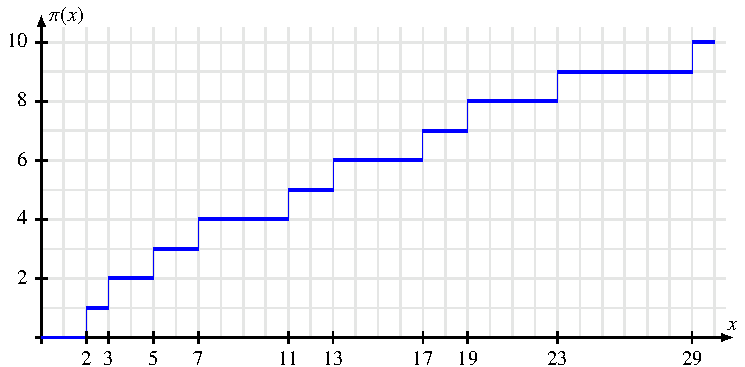
\includegraphics{papers/zeta/images/primzahlfunktion2.pdf}
    \caption{Die Primzahlfunktion von $0$ bis $30$.}
    \label{fig:zeta:primzahlfunktion}
\end{figure}

Der grundlegende Zusammenhang der Primzahlen und der Zeta-Funktion wird im ersten Abschnitt \ref{zeta:section:eulerprodukt} über das Eulerprodukt gezeigt.
\index{Primzahl}%
\index{Eulerprodukt}%
Danach folgt die Verbindung zur bereits bekannten Gamma-Funktion in Abschnitt \ref{zeta:section:zusammenhang_mit_gammafunktion}.
Schlussendlich folgt die Beschreibung der analytischen Fortsetzung die gesamte komplexe Ebene in Abschnitt \ref{zeta:section:analytische_fortsetzung}.

Diese analytische Fortsetzung wird für die Riemannsche Vermutung benötigt, ermöglicht aber auch andere interessante Aussagen.
So findet sich zum Beispiel immer wieder die aberwitzige Behauptung, das die Summe aller natürlichen Zahlen
\index{Summer aller natürlichen Zahlen}%
\begin{equation*}
    \sum_{n=1}^{\infty} n
    =
    \sum_{n=1}^{\infty}
    \frac{1}{n^{-1}}
    =
    -\frac{1}{12}
\end{equation*}
sei.
Obwohl diese Behauptung offensichtlich falsch ist, hat sie doch ihre Berechtigung, wie durch die analytische Fortsetzung gezeigt werden wird.

Die folgenden mathematischen Herleitungen sind, sofern nicht anders gekennzeichnet, eigene Darstellungen basierend auf den überaus umfangreichen Wikipedia-Artikeln auf Deutsch \cite{zeta:online:wiki_de} und Englisch \cite{zeta:online:wiki_en} sowie einer Video-Playlist \cite{zeta:online:mryoumath}.
